\documentclass[twocolumn]{article}
\usepackage[utf8]{inputenc}
\usepackage{graphicx}
\usepackage{fancyhdr}

\pagestyle{fancy}
\fancyhf{}
\cfoot{\thepage}
\rhead{Marta Lønne Jensen}
\lhead{Exponential function}

\begin{document}

\section{Introduction}

The exponential function is a function denoted by

\begin{equation}
	\exp(x) = e^x
\end{equation}

The exponential function grows faster and faster as $x$ grows. For negative $x$, the function will near 0, but never cross it.

The inverse of the exponential function is the natural logarithm, $\ln(x)$.


\section{Implementation}

This report uses a "quick and dirty" implementation of the exponential function, given as

\begin{equation}
\label{eq:imp}
	f(x) = 1 + x + \frac{x^2}{2} + \frac{x^3}{3} + ... + \frac{x^{10}}{10}
\end{equation}

The exponential function can be characterized as a power series, when looking at real numbers,

\begin{equation}
	\exp(x) = \sum_{k=0}^{\infty} \frac{x^k}{k!}
\end{equation}

which, for $k = 0$ to $k=10$, is exactly $f(x)$. This is a lot of terms and should function nicely in many cases. 

But for $x>\frac{1}{8}$, $ f(x/2)^2$ is calculated instead. This is because our implementation is a power series around zero, so values far from zero, will be more incorrect. Instead, we divide the $x$ value with two, calculate the exponential and then take it to the power of two. For the exponential function, this is the same. 

\section{Test}

As can be seen in fig. \ref{fig:exp}, the implementation is working. The two functions are exactly on top of each other. The precision of the implementation compared to the exponential function is of the order of $10^{-16}$ for $x \sim 1$, while for $x\sim 9$ it is of the order $10^{-10}$, obviously becoming less and less precise, but still well within the accepted area, while the relative precision goes from $10^{-17}$ to $10^{-15}$, indicating even less of a difference, when you take the size of the numbers into account.

\begin{figure}
	\centering
	\label{fig:exp}
	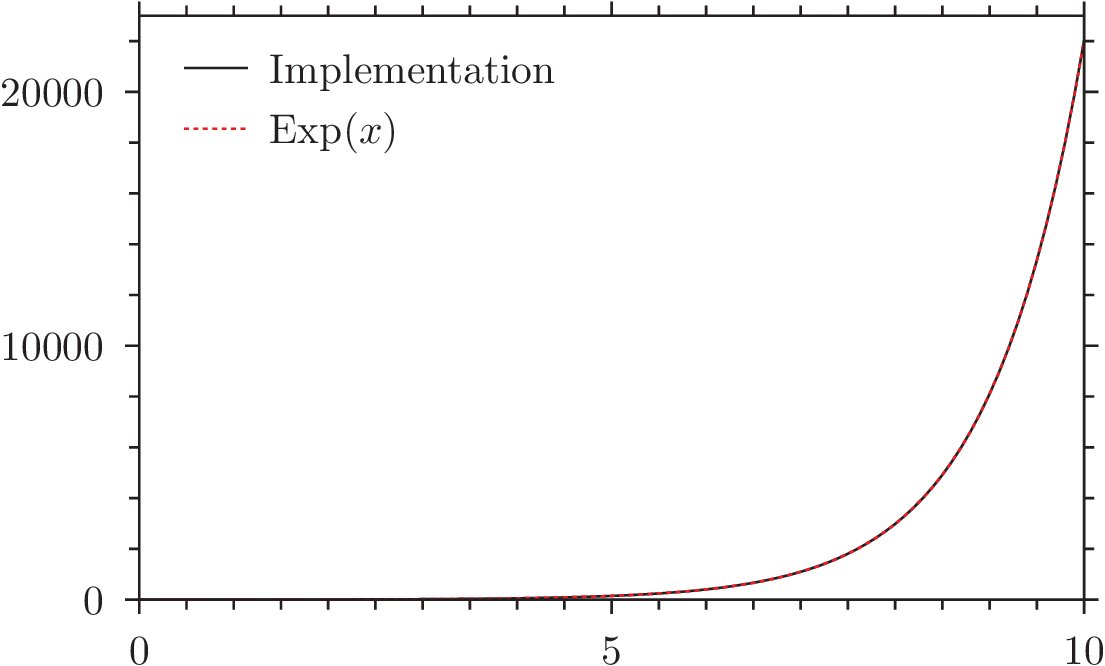
\includegraphics[width=\linewidth]{exp.png}
	\caption{The solid, black line is the implementation, eq. (\ref{eq:imp}), while the red dashed line in the exponential function.}
\end{figure}
\end{document}
